\chapter{Markov Decision Process}

\paragraph{Example}

To help conceptualize Finite Markov Processes, let us consider a simple example of changes in inventory at a store. Assume you are the store manager and that you are tasked with controlling the ordering of inventory from a supplier. Let us focus on the inventory of a particular type of bicycle. Assume that each day there is random (non-negative integer) demand for the bicycle with the probabilities of demand following a Poisson distribution (with Poisson parameter $\lambda \in \mathbb{R}_{\geq 0}$), i.e. demand $i$ for each $i = 0, 1, 2, \ldots$ occurs with probability
$$f(i) = \frac {e^{-\lambda} \lambda^i} {i!}$$
Denote $F: \mathbb{Z}_{\geq 0} \rightarrow [0, 1]$ as the Poisson cumulative probability distribution function, i.e.,
 $$F(i) = \sum_{j=0}^i f(j)$$
 \begin{itemize}
	 \item Assume you have storage capacity for at most $C \in \mathbb{Z}_{\geq 0}$ bicycles in your store. 
	 \item Each evening at 6pm when your store closes, you have the choice to order a certain number of bicycles from your supplier (including the option to not order any bicycles on a given day). 
	 \item The ordered bicycles will arrive 36 hours later (at 6am the day after the day after you order—we refer to this as delivery lead time of 36 hours). 
	 \item Denote the State at 6pm store-closing each day as $(\alpha, \beta)$, where $\alpha$ is the inventory in the store (referred to as On-Hand Inventory at 6pm) and $\beta$ is the inventory on a truck from the supplier (that you had ordered the previous day) that will arrive in your store the next morning at 6am ($\beta$ is referred to as On-Order Inventory at 6pm). Due to your storage capacity constraint of at most $C$ bicycles, your ordering policy is to order $C-(\alpha + \beta)$ if $\alpha + \beta < C$ and to not order if $\alpha + \beta \geq C$. The precise sequence of events in a 24-hour cycle is:
 \end{itemize}
 
In sum,
\begin{itemize}
	\item Observe the $(\alpha, \beta)$ \textit{State} at 6pm store-closing (call this state $S_t$).
	\item Immediately order according to the ordering policy described above.
	\item Receive bicycles at 6am if you had ordered 36 hours ago.
	\item Open the store at 8am.
	\item Experience random demand from customers according to demand probabilities stated above (number of bicycles sold for the day will be the minimum of demand on the day and inventory at store opening on the day).
	\item Close the store at 6pm and observe the state (this state is $S_{t+1}$).
\end{itemize}

If we let this process run for a while, in steady-state, we ensure that $\alpha + \beta \leq C$. So to model this process as a Finite Markov Process, we shall only consider the steady-state (finite) set of states
$$\mathcal{S} = \{(\alpha, \beta) | \alpha \in \mathbb{Z}_{\geq 0}, \beta \in \mathbb{Z}_{\geq 0}, 0 \leq \alpha + \beta \leq C\}$$
So restricting ourselves to this finite set of states, our order quantity equals $C - (\alpha + \beta)$ when the state is $(\alpha, \beta)$.

If the current state $S_t$ is $(\alpha, \beta)$, there are only $\alpha + \beta + 1$ possible next states $S_{t+1}$ as follows\footnotemark:
$$(\alpha + \beta - i, C - (\alpha + \beta)) \text{ for } i =0, 1, \ldots, \alpha + \beta$$
with transition probabilities governed by the Poisson probabilities of demand as follows:
\begin{align*}
	&\mathcal{P}((\alpha, \beta), (\alpha + \beta - i, C - (\alpha + \beta))) = f(i)\text{ for } 0 \leq i \leq \alpha + \beta - 1\\
	&\mathcal{P}((\alpha, \beta), (0, C - (\alpha + \beta))) = \sum_{j=\alpha+\beta}^{\infty} f(j) = 1 - F(\alpha + \beta - 1)
\end{align*}
\begin{itemize}
	\item $P((\alpha, \beta), (\alpha + \beta - i, C - (\alpha + \beta)))$ is the probability of transitioning from state $(\alpha, \beta)$ to $(\alpha + \beta - i, C - (\alpha + \beta))$ when demand equals $i$. The probability $f(i)$ is based on the Poisson demand distribution.
	\item If demand exceeds $\alpha + \beta$, the system transitions to a state where all on-hand inventory is depleted:
		\begin{align*}
			\mathbb{P}((\alpha, \beta), (0, C - (\alpha + \beta))) = 1 - F(\alpha + \beta - 1)
		\end{align*}
	\item $1 - F(\alpha + \beta - 1)$ gives the probability that the demand is greater than or equal to $\alpha+\beta$ (\ie demand is large enough to deplete the entire on-hand inventory).
\end{itemize}
\footnotetext{Since $\alpha+\beta=C$, there are only $C+1$ states. Also, the number of bicycles is the sum of the number of bicycles in the inventory and the truck. Thus, the next state's bicycles is $\alpha+\beta+i$}


\section{Markov Reward Process}
% \label{sec:}
The reason we covered Markov Processes is that we want to make our way to Markov Decision Processes (the framework for Reinforcement Learning algorithms) by adding incremental features to Markov Processes. Now we cover an intermediate framework between Markov Processes and Markov Decision Processes, known as Markov Reward Processes. We essentially just include the notion of a numerical reward to a Markov Process each time we transition from one state to the next. These rewards are random, and all we need to do is to specify the probability distributions of these rewards as we make state transitions.

The main purpose of Markov Reward Processes is to calculate how much reward we would accumulate (in expectation, from each of the non-terminal states) if we let the process run indefinitely, bearing in mind that future rewards need to be discounted appropriately (otherwise, the sum of rewards could blow up to $\infty$). In order to solve the problem of calculating expected accumulative rewards from each non-terminal state, we will first set up some formalism for Markov Reward Processes, develop some (elegant) theory on calculating rewards accumulation, write plenty of code (based on the theory), and apply the theory and code to the simple inventory example (which we will embellish with rewards equal to negative of the costs incurred at the store).

Formally, A Markov Reward Process is a Markov Process, along with a time-indexed sequence of Reward random variables $R_t\in \mathcal{D}$ (countable set $\mathcal{D}$) for time steps $t=1,2,\dots,$ satisfying the Markov Property (including Rewards):
$$P[(R_{t+1}, S_{t+1})|S_t, S_{t-1}, \dots , S_0] = P[(R_{t+1}, S_{t+1})|S_t]\  \forall t\geq 0.$$
In reinforcement learning, a MRP arises when you fix a policy $\pi$ for your MDP. Then all the decision making is accounted for, and we have a MRP with the induced transition kernel
\begin{align*}
	v(s)&=\mathbb{E}[G_t|S_t=s]\\
		&=\mathbb{E}\left[\sum_{k=0}^\infty \gamma^kR_{t+k+1}|S_t=s\right]\\
		&= \sum_{s',r}p(s',r|s)[r+\gamma v(s')]
\end{align*} 
Bellman equation for MRP. In matrix form,
$$v = PR+\gamma Pv.$$
We can solve this system by
$$v = (I-\gamma P)^{-1}PR$$
An MRP is fully characterized by a $\langle S,P,R,\gamma \rangle$ tuple, where $S$ is a set of states, $P$ is a transition probability matrix, $R$ is a reward function, and $\gamma\in[0,1]$  is a discount factor. I will explain more about the discount factor later. 


\section{Markov Decision Process}
% \label{sec:}

The general framework of MDPs (representing environments as MDPs) allows us to model virtually any complex sequential decision-making problem under uncertainty in a way that RL agents can interact with and learn to solve solely through experience. 

\begin{figure}[h]
	\centering
	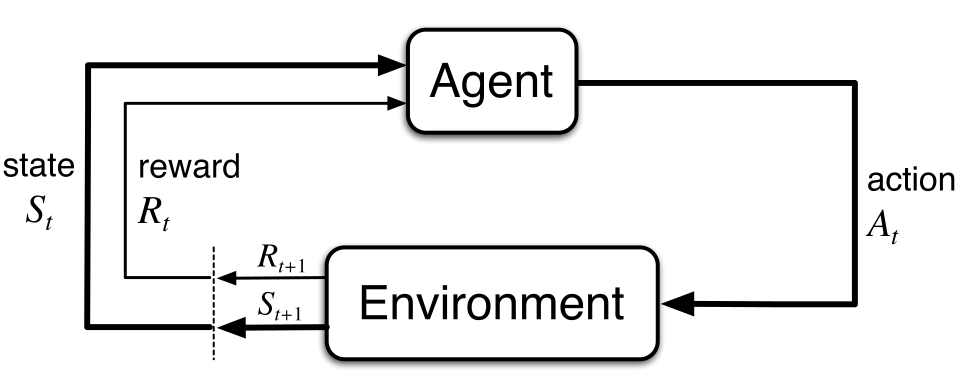
\includegraphics[scale=0.3]{./images/mdp.png}
	\caption{The agent-environment interaction in a Markov decision process.}
	\label{fig:mdp_ill}
\end{figure}

Components of RL:
\begin{itemize}
	\item An agent
	\item A policy
	\item A reward signal: what is good in an immediate sense.
	\item A value function: what is good in the long run.
	\item A model of the environment: This allows inferences to be made about how the environment will behave.
\end{itemize}
An MDP is fully characterized by a $\langle S,A,P,R,\gamma \rangle$ tuple, where $S$ is a set of states, $P$ is a transition probability matrix, $R$ is a reward function, and $\gamma\in[0,1]$  is a discount factor.

\begin{definition}[Markov Property]
	A state $S_t$ is \textbf{Markov} if and only if 
	$$P[S_{t+1}|S_t, A_t] = P[S_{t+1}|S_t, A_t, S_{t-1},A_{t-1},...]$$
\end{definition}
\begin{itemize}
	\item Actions: a mechanism to influence the environment
	\item State: specific configurations of the environment
\end{itemize}

\begin{definition}[Transition Function]
	$$p(s',r|s,a) = P(S_t=s',R_t=r|S_{t-1}=s,A_{t-1}=a)$$
\end{definition}
\begin{itemize}
	\item The way the environment changes as a response to actions is referred to as the state-transition probabilities, or more simply, the transition function, and is denoted by $T(s,a,s')$.
	\item $\sum_{r\in \mathcal{R}}\sum_{s'\in \mathcal{S}}p(s',r|s,a) = 1, \quad \forall s \in \mathcal{S}, \forall a\in \mathcal{A}(s)$
	\item $p(s'|s,a)=P(S_t=s'|S_{t-1}=s,A_{t-1}=a)=\sum_{r\in \mathcal{R}}p(s',r|s,a)$
\end{itemize}

\begin{definition}[Reward Hypothesis]
	All goals can be described by the maximization of expected cumulative reward.
\end{definition}
\begin{itemize}
	\item All goals and purposes can be well thought of as the maximization of the expected value of the cumulative sum of a received scalar signal (\ie reward).
\end{itemize}

\begin{definition}[Reward Function]
	\begin{align*}
		r(s,a)&= \mathbb{E}[R_t|S_{t-1}=s,A_{t-1}=a]\\
		&= \sum_{r\in \mathcal{R}}r\sum_{s'\in \mathcal{S}}p(s',r|s,a)
	\end{align*}
\end{definition}
\begin{itemize}
	\item $R_t\in \mathcal{R} \subset \mathbb{R}.$ 
		\begin{itemize}
			\item Note that negative reward is still reward.
		\end{itemize}
	\item The expected reward function is defined as a function that takes in a state-action pair.
	\item It is the expectation of reward at time step $t$, given the state-action pair in the previous time step.
	\item The reward function can also be defined as a function that takes a full transition tuple $s,a,s'$.
		\begin{align*}
			r(s,a,s')&= \mathbb{E}[R_t|S_{t-1}=s,A_{t-1}=a,S_{t}=s]\\
			&= \sum_{r\in \mathcal{R}}r\frac{p(s',r|s,a)}{p(s'|s,a)}
		\end{align*}
\end{itemize}

\begin{definition}[Discount Factor, $\gamma$]
	$$G_t = R_{t+1}+\gamma R_{t+2}+\gamma^2 R_{t+3}+\cdots+\gamma^{T-1} R_{T} $$
\end{definition}

\begin{itemize}
	\item The sum of all rewards obtained during the course of an episode is referred to as the \textit{return}, $G_t$.
	\item Episodic tasks: $G_t = R_{t+1} + R_{t+2} + \cdots + R_{T}.$
		\begin{itemize}
			\item $G_t = R_{t+1}+\gamma G_{t+1}$
		\end{itemize}
	\item Continuing tasks: $G_t = R_{t+1} + \gamma R_{t+2} +  \gamma^2 R_{t+3} \cdots =\sum_{k=0}^{\infty} \gamma^{k} R_{t+k+1}.$
		\begin{itemize}
			\item $\gamma=0$: myopic evaluation
			\item $\gamma=1$: far-sighted evaluation
			\item Uncertainty about the future that may not be fully observed
			\item Mathematically convenient to discount rewards. 
			\item Avoid infinite returns in cyclic Markov processes.
		\end{itemize}
\end{itemize}

\paragraph{A Simple Example:}
\begin{itemize}
	\item Environment:
		\begin{itemize}
			\item The grid world has 3 states: $S1$, $S2$, and $S3$.
			\item The agent can take actions $A=\{left,right\}$.
			\item The rewards are as follows:
				\begin{itemize}
					\item $R_{left}=-1$: penalty for moving left
					\item $R_{right}=+1$: reward for moving right
				\end{itemize}
			\item The discount factor $\gamma$: 0.9.
		\end{itemize}
	\item Episode:
		\begin{enumerate}
			\item The agent starts in $S1$.
			\item If the agent moves left, it incurs a penalty ($R_{left}=-1$), and the episode ends.
			\item If the agent moves right, it receives a reward ($R_{right}=+1$), transitions to $S2$, and the episode continues.
			\item In $S2$, the agent faces the same choices.
			\item The episode ends when the agent either moves left or reaches $S3$.
		\end{enumerate}
	\item Return Calculation:
		\begin{itemize}
			\item Let's calculate the return for a sample trajectory: $\{S1,right,S2,right,S3\}$.
			\item $G=R_{right}+\gamma R_{right}+\gamma^2R_{right}=2.71$ 
			\item So, the return for this trajectory is 2.71.
		\end{itemize}
\end{itemize}

\section{Policies and Value Functions}
\begin{itemize}
	\item Policies are universal plans, which provides all possible plans for all states. 
		\begin{itemize}
			\item Plans are not enough to fully describe an environment in stochastic environments.
				\begin{itemize}
					\item What if an agent intends to move right, but ends up going left. Which action does the agent take?
				\end{itemize}
			\item Policies are the per-state action descriptions.
			\item Policy can be stochastic or deterministic.
			\item A policy is a function that prescribes actions to take for a given non-terminal state.
		\end{itemize}
\end{itemize}

Formally, a policy is a mapping from states to probabilities of selecting each possible action. It can be defined 
$$\pi(a|s)$$

\subsection{The State-Value Functions}

Almost all reinforcement learning algorithms involve estimating \textit{value functions}, functions of states (or of state-action pairs) that estimate how good it is for the agent to be in a given state (or how good it is to perform a given action in a given state). The notion of ``how good'' here is defined in terms of future rewards that can be expected, or, to be precise, in terms of \textbf{expected return}. Sure, we want high returns, but high in expectation (on average). Of course, the rewards the agent can expect to receive in the future depend on what actions it will take. Accordingly, value functions are defined with respect to particular ways of action, called policies. 

\begin{definition}[The State-Value Function, $V$]
	The state-value function $v(s)$ for policy $\pi$ of an Markov Reward Process is the expected return starting from state $s$
	\begin{align*}
		v_{\pi}(s) &= \mathbb{E}_\pi[G_t|S_t=s]\\
				   &= \mathbb{E}_\pi \Bigg[\sum_{k=0}^\infty \gamma^kR_{t+1+k}\Big|S_t=s\Bigg], \quad \forall s\in \mathcal{S}
				   % &= \mathbb{E}_\pi \Bigg[R_{t+1}+\gamma G_{t+1}\sum_{k=1}^\infty \gamma^kR_{t+1+k}\Big|S_t=s\Bigg], \quad \forall s\in \mathcal{S}\\
	\end{align*}
	$$$$
\end{definition}

\begin{itemize}
	\item The value of a state $s$ is the expectation over policy $\pi$.
	\item Value function is the expected return. 
		\begin{itemize}
			\item Reward: one-step signal that an agent receives.
			\item Return: total discounted rewards, which is the sum of rewards obtained from time $t$ onward.
		\end{itemize}
	\item If we are given a policy and the MDP, we should be able to calculate the expected return starting from every single state. 
\end{itemize}

The state-value function satisfies the \textit{Bellman equation}, which expresses the relationship between the value of a state and the values of its successor states:
\begin{align}
	v_\pi(s) &= \mathbb{E}_\pi[G_t|S_t=s]\\
	& = \mathbb{E}_\pi[R_{t+1} + \gamma G_{t+1}|S_t=s]\\
	% & = \mathbb{E}_\pi[R_{t+1} + \gamma v(s_{t+1})|S_t=s]\\
	& = \sum_{a}\pi(a|s)\sum_{s',r}p(s',r|s,a)[r + \gamma v_\pi(s')],\, \forall s \in \mathcal{S}.
	\label{eq:state_value_bellman}
\end{align}
For better understanding, let's look at the \Cref{fig:state_value_diagram}. Starting from state $s$, the root node at the top, the agent could take any of some set of actions (three actions are shown in the diagram), based on its policy $\pi$. From each of these, the environment could respond with one of several next states, $s'$ (two states are shown in the figure), along with a reward, $r$, depending on its dynamics given by the function $p$. The Bellman equation averages over all the possibilities, weighting each by its probability of occurring. \textbf{It states that the value of the start state must equal (discounted) the value of the expected next state, plus the reward expected along the way}. 
\begin{figure}[h]
	\centering
	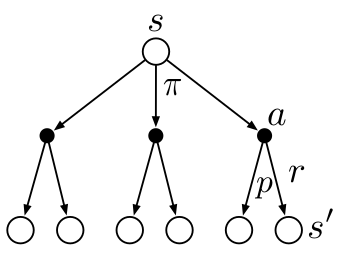
\includegraphics[scale=0.3]{./images/backup_vpi.png}
	\label{fig:state_value_diagram}
\end{figure}
The derivation of \Cref{eq:state_value_bellman} is given in \Cref{appendix:bellman_equation}. The state-value function is essential for understanding the value of different states in a Markov Decision Process (MDP) and is often used in various reinforcement learning algorithms, such as value iteration and policy iteration.

% The Bellman equation for the state-value function can be expressed in matrix form as follows:
% \begin{align}
% 	v_\pi(s) &= \mathbb{E}_\pi[G_t|S_t=s]\\
% 	& = \mathbb{E}_\pi[R_{t+1} + \gamma G_{t+1}|S_t=s]\\
% 	& = \mathbb{E}_\pi[R_{t+1} + \gamma v(s_{t+1})|S_t=s]\\
% 	% & = \sum_{a}\pi(a|s)\sum_{s',r}p(s',r|s,a)[r + \gamma v_\pi(s')],\, \forall s \in \mathcal{S}.
% 	% \label{eq:state_value_bellman}
% \end{align}




\subsection{The Action-Value Function}
\begin{itemize}
	\item Another critical question that we often need to ask is not merely about the value of a state but the value of taking action $a$ at a state $s$.
	\item Which action is better under each policy?
	\item The action-value function, also known as $Q$-function or $Q^\pi(s,a)$, captures precisely this.
		\begin{itemize}
			\item The expected return if the agent follows policy $\pi$ after taking action $a$ in state $s$.
		\end{itemize}
\end{itemize}

\begin{definition}[The Action-Value Function, $Q$]
	The action-value function $q_{\pi}(s,a)$ for policy $\pi$ is the expected return starting from state $s$, tacking action $a$ under policy $\pi$
	$$q_{\pi}(s,a) = \mathbb{E}_\pi[G_t|S_t=s, A_t=a]=\mathbb{E}_\pi\Bigg[\sum_{k=0}^{\infty}\gamma^k R_{t+k+1}\Bigg| S_t=s, A_t=a\Bigg]$$
\end{definition}

\begin{itemize}
	\item The Bellman equation for the action-value function is given by
	\begin{align*}
		q_{\pi}(s,a) &= \mathbb{E}_\pi[G_t|S_t=s, A_t=a]\\
		& = \mathbb{E}_\pi[R_{t+1} + \gamma G_{t+1}|S_t=s, A_t=a]\\
		& = \sum_{s',r}p(s',r|s,a)[r + \gamma v_\pi(s')]
	\end{align*}
	\item Notice that we do not weight over actions because we are interested only in a specific action.
	\item The action-value function is crucial for understanding the value of different state-action pairs in a Markov Decision Process (MDP) and is used in various reinforcement learning algorithms, such as Q-learning and deep Q-networks (DQN).
	\item The derivation is given in \Cref{appendix:bellman_equation}
\end{itemize}

The state-value function can be also expressed by using the action-value function as follows:
\begin{align*}
	v_\pi(s) &= \mathbb{E}_{\pi}[G_t|S_t = s]\\ 
	&= \sum_{g_t} g_t\cdot P[G_t|S_t=s]\\
	&= \sum_{g_t} g_t\cdot P[G_t,S_t=s]/P[S_t=s]\\
	&= \sum_{g_t} g_t\cdot \sum_a P[G_t,S_t=s, A_t=a]/P[S_t=s]\\
	&= \sum_{g_t} g_t\cdot \sum_a \Big[P[G_t|S_t=s, A_t=a]P[S_t=s, A_t=a]\Big]/P[S_t=s]\\
	%&= \sum_{g_t} g_t \sum_a P(G_t|S_t=s, A_t=a) P(A_t=a|S_t=s)\\
	&= \sum_{g_t} g_t \sum_a P[G_t, A_t=a|S_t=s] P[A_t=a|S_t=s]\\
	&= \sum_{a} \sum_{g_t} g_t P[G_t|S_t=s, A_t=a] P[A_t=a|S_t=s]\\
	&= \sum_{a} q_\pi(s,a) \pi(a|s)
\end{align*}
Note that the expectation is parameerized $\pi$ as written in $\mathbb{E}_{\pi}$. We can also simply prove it by the \textit{Law of Total Expectation} \footnote{
$\mathbb{E}[\mathbb{E}[X|Y]] = \sum_{y}\Big[\sum_{x}x\cdot\ p(X=x|Y)\Big] p(Y=y) = \mathbb{E}[X]$},
\begin{align*}
	v_\pi(s) &= \mathbb{E}_{\pi}[G_t|S_t = s]\\ 
	&= \mathbb{E}[\mathbb{E}_{\pi}[G_t|S_t=s, A_t=a]]\\
	&= \sum_{a} \mathbb{E}_{\pi}[G_t|S_t=s, A_t=a] P(A_t = a|S_t = s)\\
	&= \sum_{a} q_\pi(s,a) \pi(a|s)
\end{align*}
An intuitive explantation of this derivation is that the expectation depends on an action $a\sim \pi(a|s)$. We want to estimate the expected total return by the sampled action (this is because the total return is the function of $a$, implicitly). Then, we need to introduce an action variable $a$ and its probability in the expression as the second line of the equation. 

\subsection{The Action-Advantage Function}

\begin{definition}[The Action-Advantage Function, $A$]
	$$a_{\pi}(s,a) = q_\pi(s,a)-v_\pi(s)$$
\end{definition}

The advantage function describes how much better it is to take action $a$ instead of following policy $\pi$. In other words, the advantage of choosing action $a$ over the default action, set by the policy.

\section{Optimality}

Solving a reinforcement learning task means, roughly, finding a policy that achieves a lot of reward over the long run. For finite MDPs, we can precisely define an optimal policy in the following way. Value functions define a partial ordering over policies. A policy $\pi$ is defined to be better than or equal to a policy $\pi'$ if its expected return is greater than or equal to that of $\pi'$ for all states. In other words, $\pi\geq \pi'$ if and only if $v_\pi(s)\geq v_{\pi'}(s)$ for all $s\in \mathcal{S}$. There is always at least one policy that is better than or equal to all other policies. This is an \textit{optimal policy}. The optimal state-value function, denoted $v_*$ can be defined as 


\begin{definition}[Optimal State-Value Function]
	The optimal state-value function $v_{*}(s)$ is the maximum value over all policies
	$$v_{*}(s) = \max_{\pi} v_{\pi}(s),\quad \forall s\in \mathcal{S}.$$
\end{definition}

\begin{itemize}
	\item The optimal state-value function can be obtained as follows:
%		\begin{align*}
%			v_{*}(s)&= \max_{a\in\mathcal{A}(s)} q_*(s,a)\\
%			&= \max_a \sum_{s',r}p(s',r|s,a)[r + \gamma v_*(s')]
%		\end{align*}

		\begin{align*}
			v_*(s) &= \max_{a\in \mathcal{A}(s)}q_{\pi_*}(s,a)\\
			&= \max_a \mathbb{E}_{\pi_*}[G_t| S_t=s, A_t=a]\\
			&= \max_a \mathbb{E}_{\pi_*}[R_{t+1}+\gamma G_{t+1}| S_t=s, A_t=a]\\
			&= \max_a \mathbb{E}_{\pi_*}[R_{t+1}+\gamma v_*(S_{t+1})| S_t=s, A_t=a]\\
			&= \max_a \sum_{r,s'}p(s',r|s,a)\Big[r + \gamma  v_*(s')\Big] 
	\end{align*}

\end{itemize}

\begin{definition}[Optimal Action-Value Function]
	The optimal action-value function $q_{*}(s, a)$ is the maximum value over all policies
	$$q_{*}(s,a) = \max_{\pi} q_{\pi}(s,a), \quad \forall s\in \mathcal{S} \textrm{ and } a\in \mathcal{A}.$$
\end{definition}
\begin{itemize}
	\item The optimal action-value function can be obtained as follows:
		\begin{align*}
		q_{*}(s,a) &= \mathbb{E}[R_{t+1}+\gamma v_*(S_{t+1})|S_t=s, A_t=a]\\
		&= \sum_{s',r}p(s',r|s,a)[r + \gamma \max_a q_*(s',a')]
		\end{align*}
		\begin{figure}[h]
			\centering
			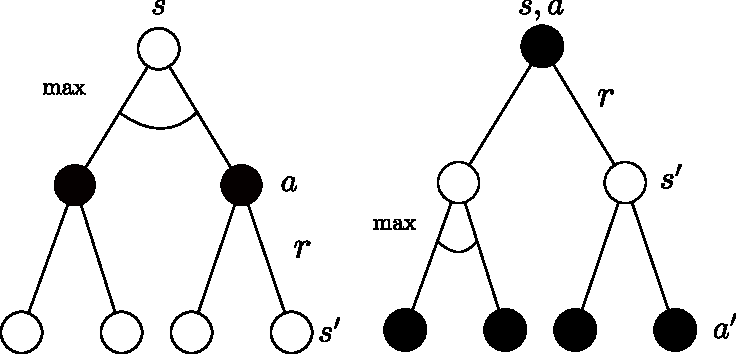
\includegraphics[scale=0.5]{./images/optimal_action.pdf}
		\end{figure}
	\item The optimal value function specifies the best possible performance in the MDP.
	\item The MDP is solved when we know the optimal value function
\end{itemize}

\begin{theorem}[Optimal Policy Theorem]
	$$\pi\geq \pi' \quad\textrm{if}\quad v_\pi(s) \geq v_{\pi'}(s), \forall s$$
	For any Markov Decision Process:
	\begin{itemize}
		\item There exists an optimal policy $\pi_*$ that is better than or equal to all other policies, $\pi_*\geq \pi, \forall \pi$
		\item All optimal policies achieve the optimal value function, $v_{\pi_*}(s) = v_*(s)$
		\item All optimal policies achieve the optimal action-value function, $q_{\pi_*}(s,a) = q_{*}(s,a)$
	\end{itemize}
\end{theorem}

An optimal policy can be found by maximizing over $q_*(s,a)$, 
\begin{align*}
	\pi_*(a|s) = 
	\begin{cases} 
		&1 \quad \textrm{if } a = \argmax_{a\in \mathcal{A}}q_*(s,a)\\
		&0 \quad \textrm{otherwise}
	\end{cases}
\end{align*}
\begin{itemize}
	\item There is always a deterministic optimal policy for any MDP
	\item If we know $q_*(s,a)$, we immediately have the optimal policy 
		\begin{itemize}
			\item Q-learning: learns Q values first
			\item Policy gradient: learns optimal policy without learning Q values
		\end{itemize}
\end{itemize}

